\chapter{Aplikacja Twitter Analyser}
\qquad asas

\begin{figure}[h] % h means here
	\centering
	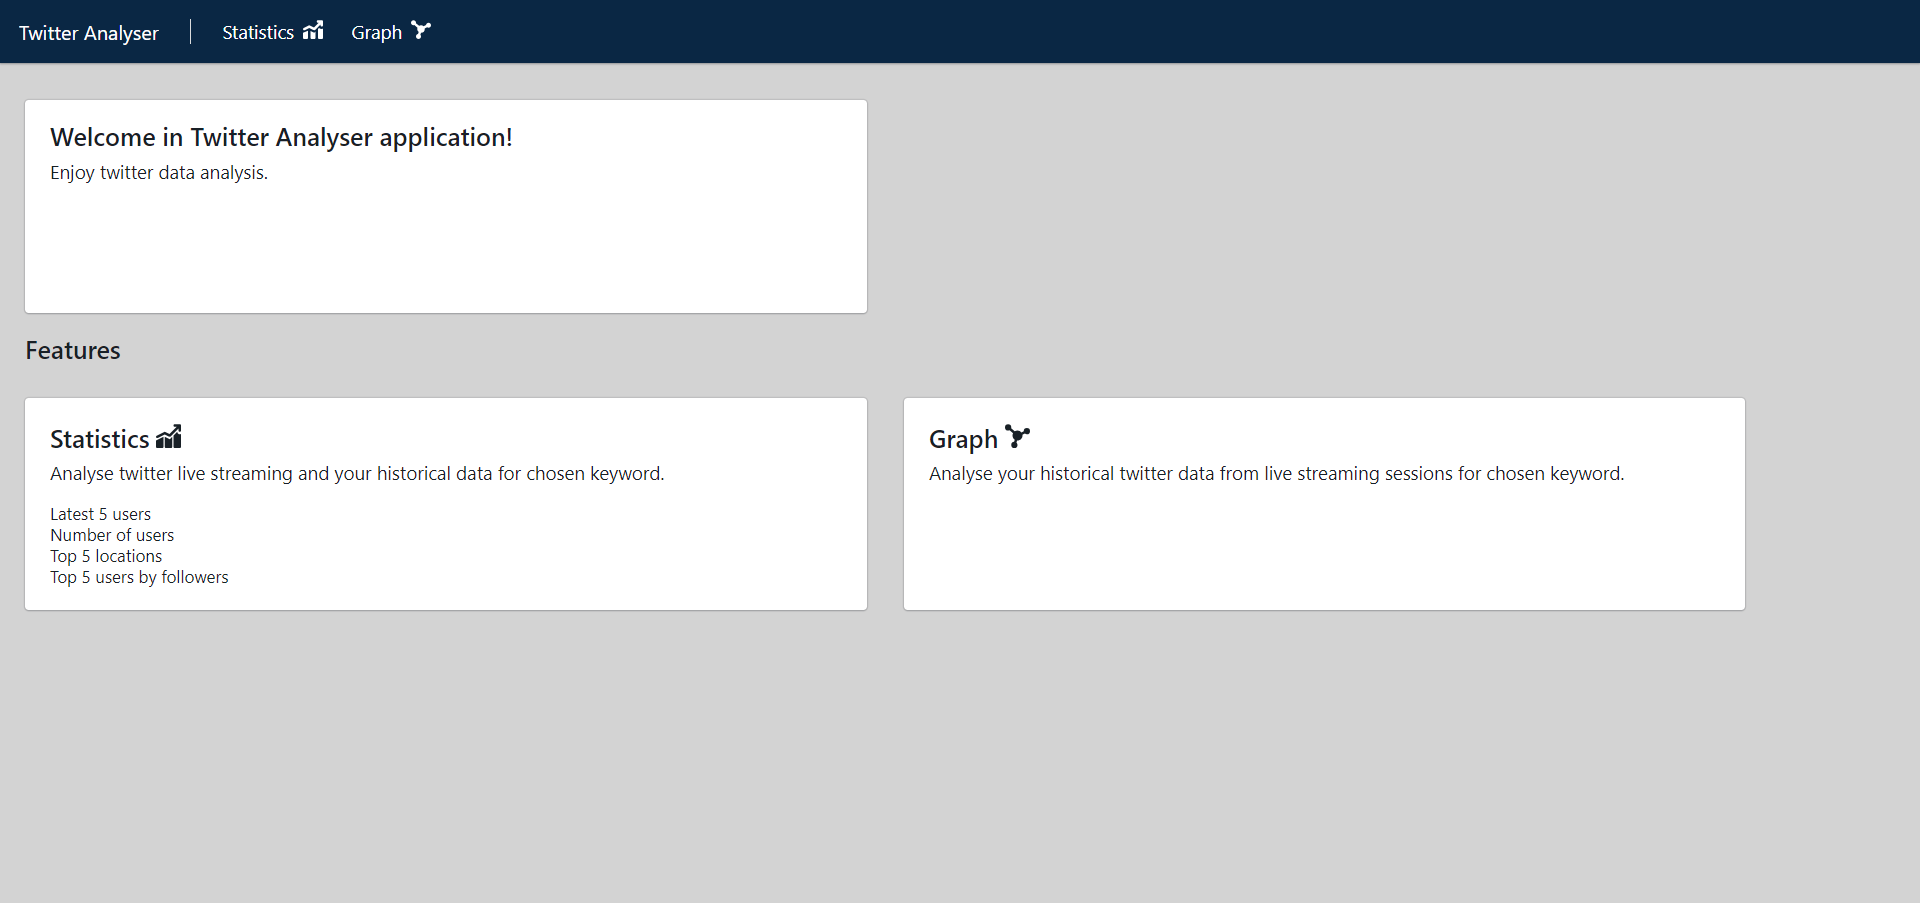
\includegraphics[width=1.0\linewidth]{img/twitter_analyser_1}
	\caption{Przykład zastosowania operacji na strumieniach oraz wyrażenia lambda w kodzie napisanym w języku Java w wersji 8.}
\end{figure}

\begin{figure}[h] % h means here
	\centering
	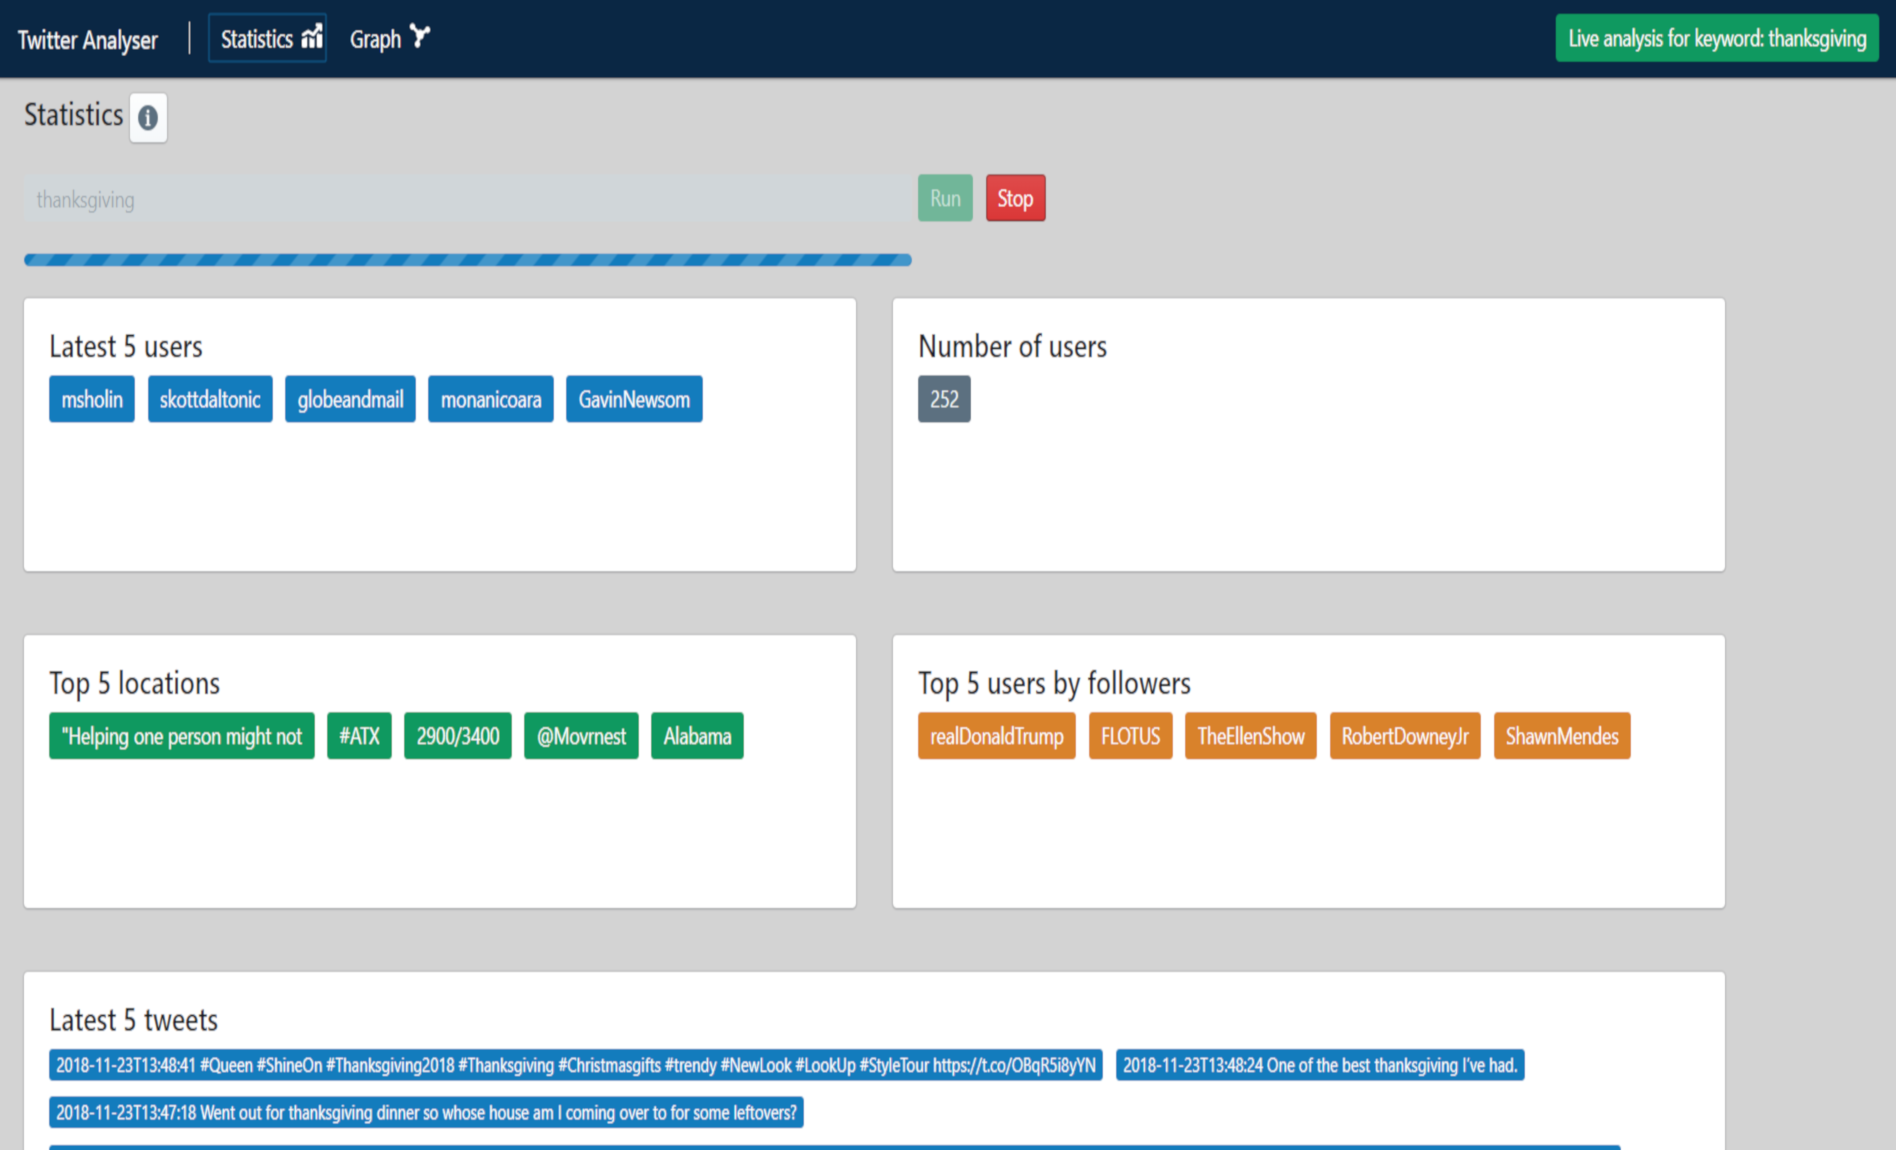
\includegraphics[width=1.0\linewidth]{img/twitter_analyser_thanks_giving_2}
	\caption{Przykład zastosowania operacji na strumieniach oraz wyrażenia lambda w kodzie napisanym w języku Java w wersji 8.}
\end{figure}

\begin{figure}[h] % h means here
	\centering
	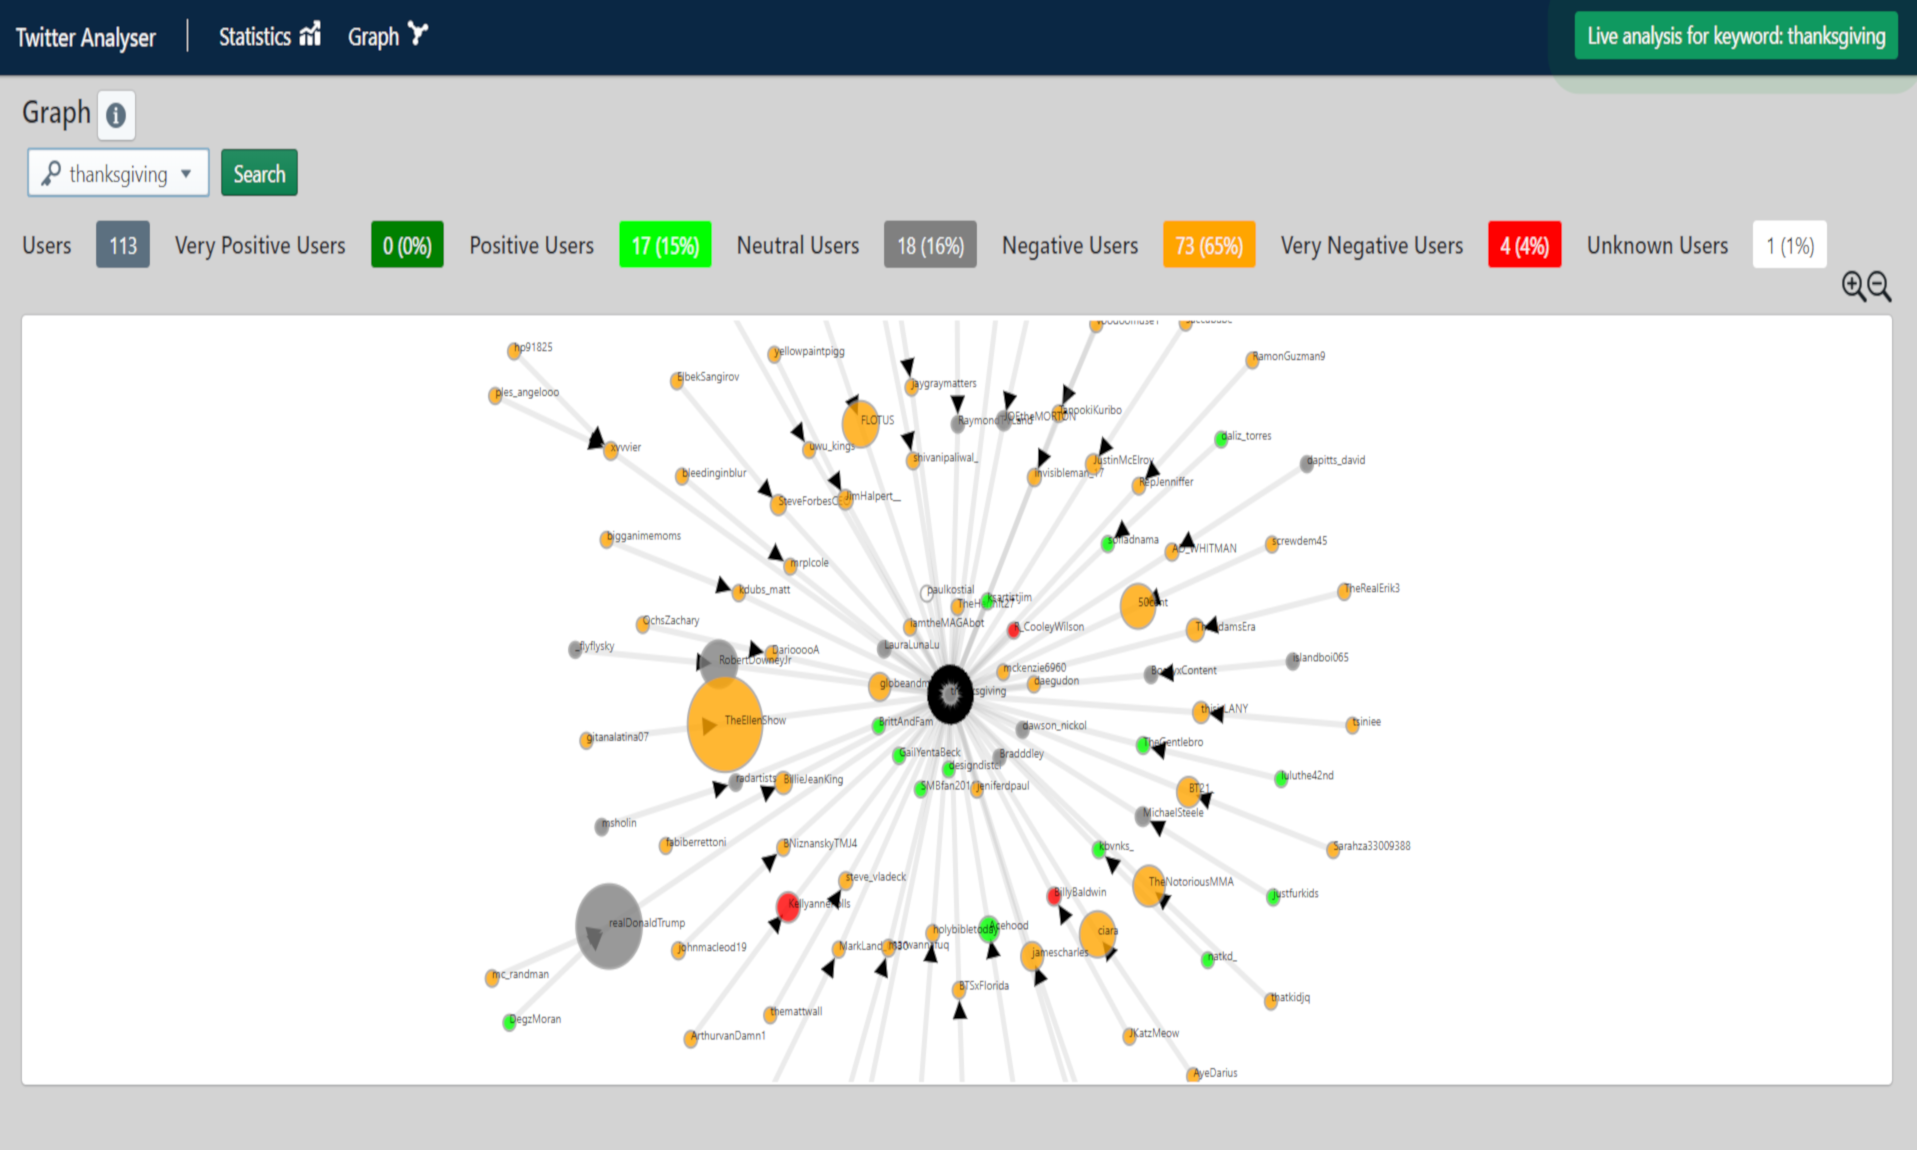
\includegraphics[width=1.0\linewidth]{img/twitter_analyser_thanks_giving_1}
	\caption{Przykład zastosowania operacji na strumieniach oraz wyrażenia lambda w kodzie napisanym w języku Java w wersji 8.}
\end{figure}

\begin{figure}[h] % h means here
	\centering
	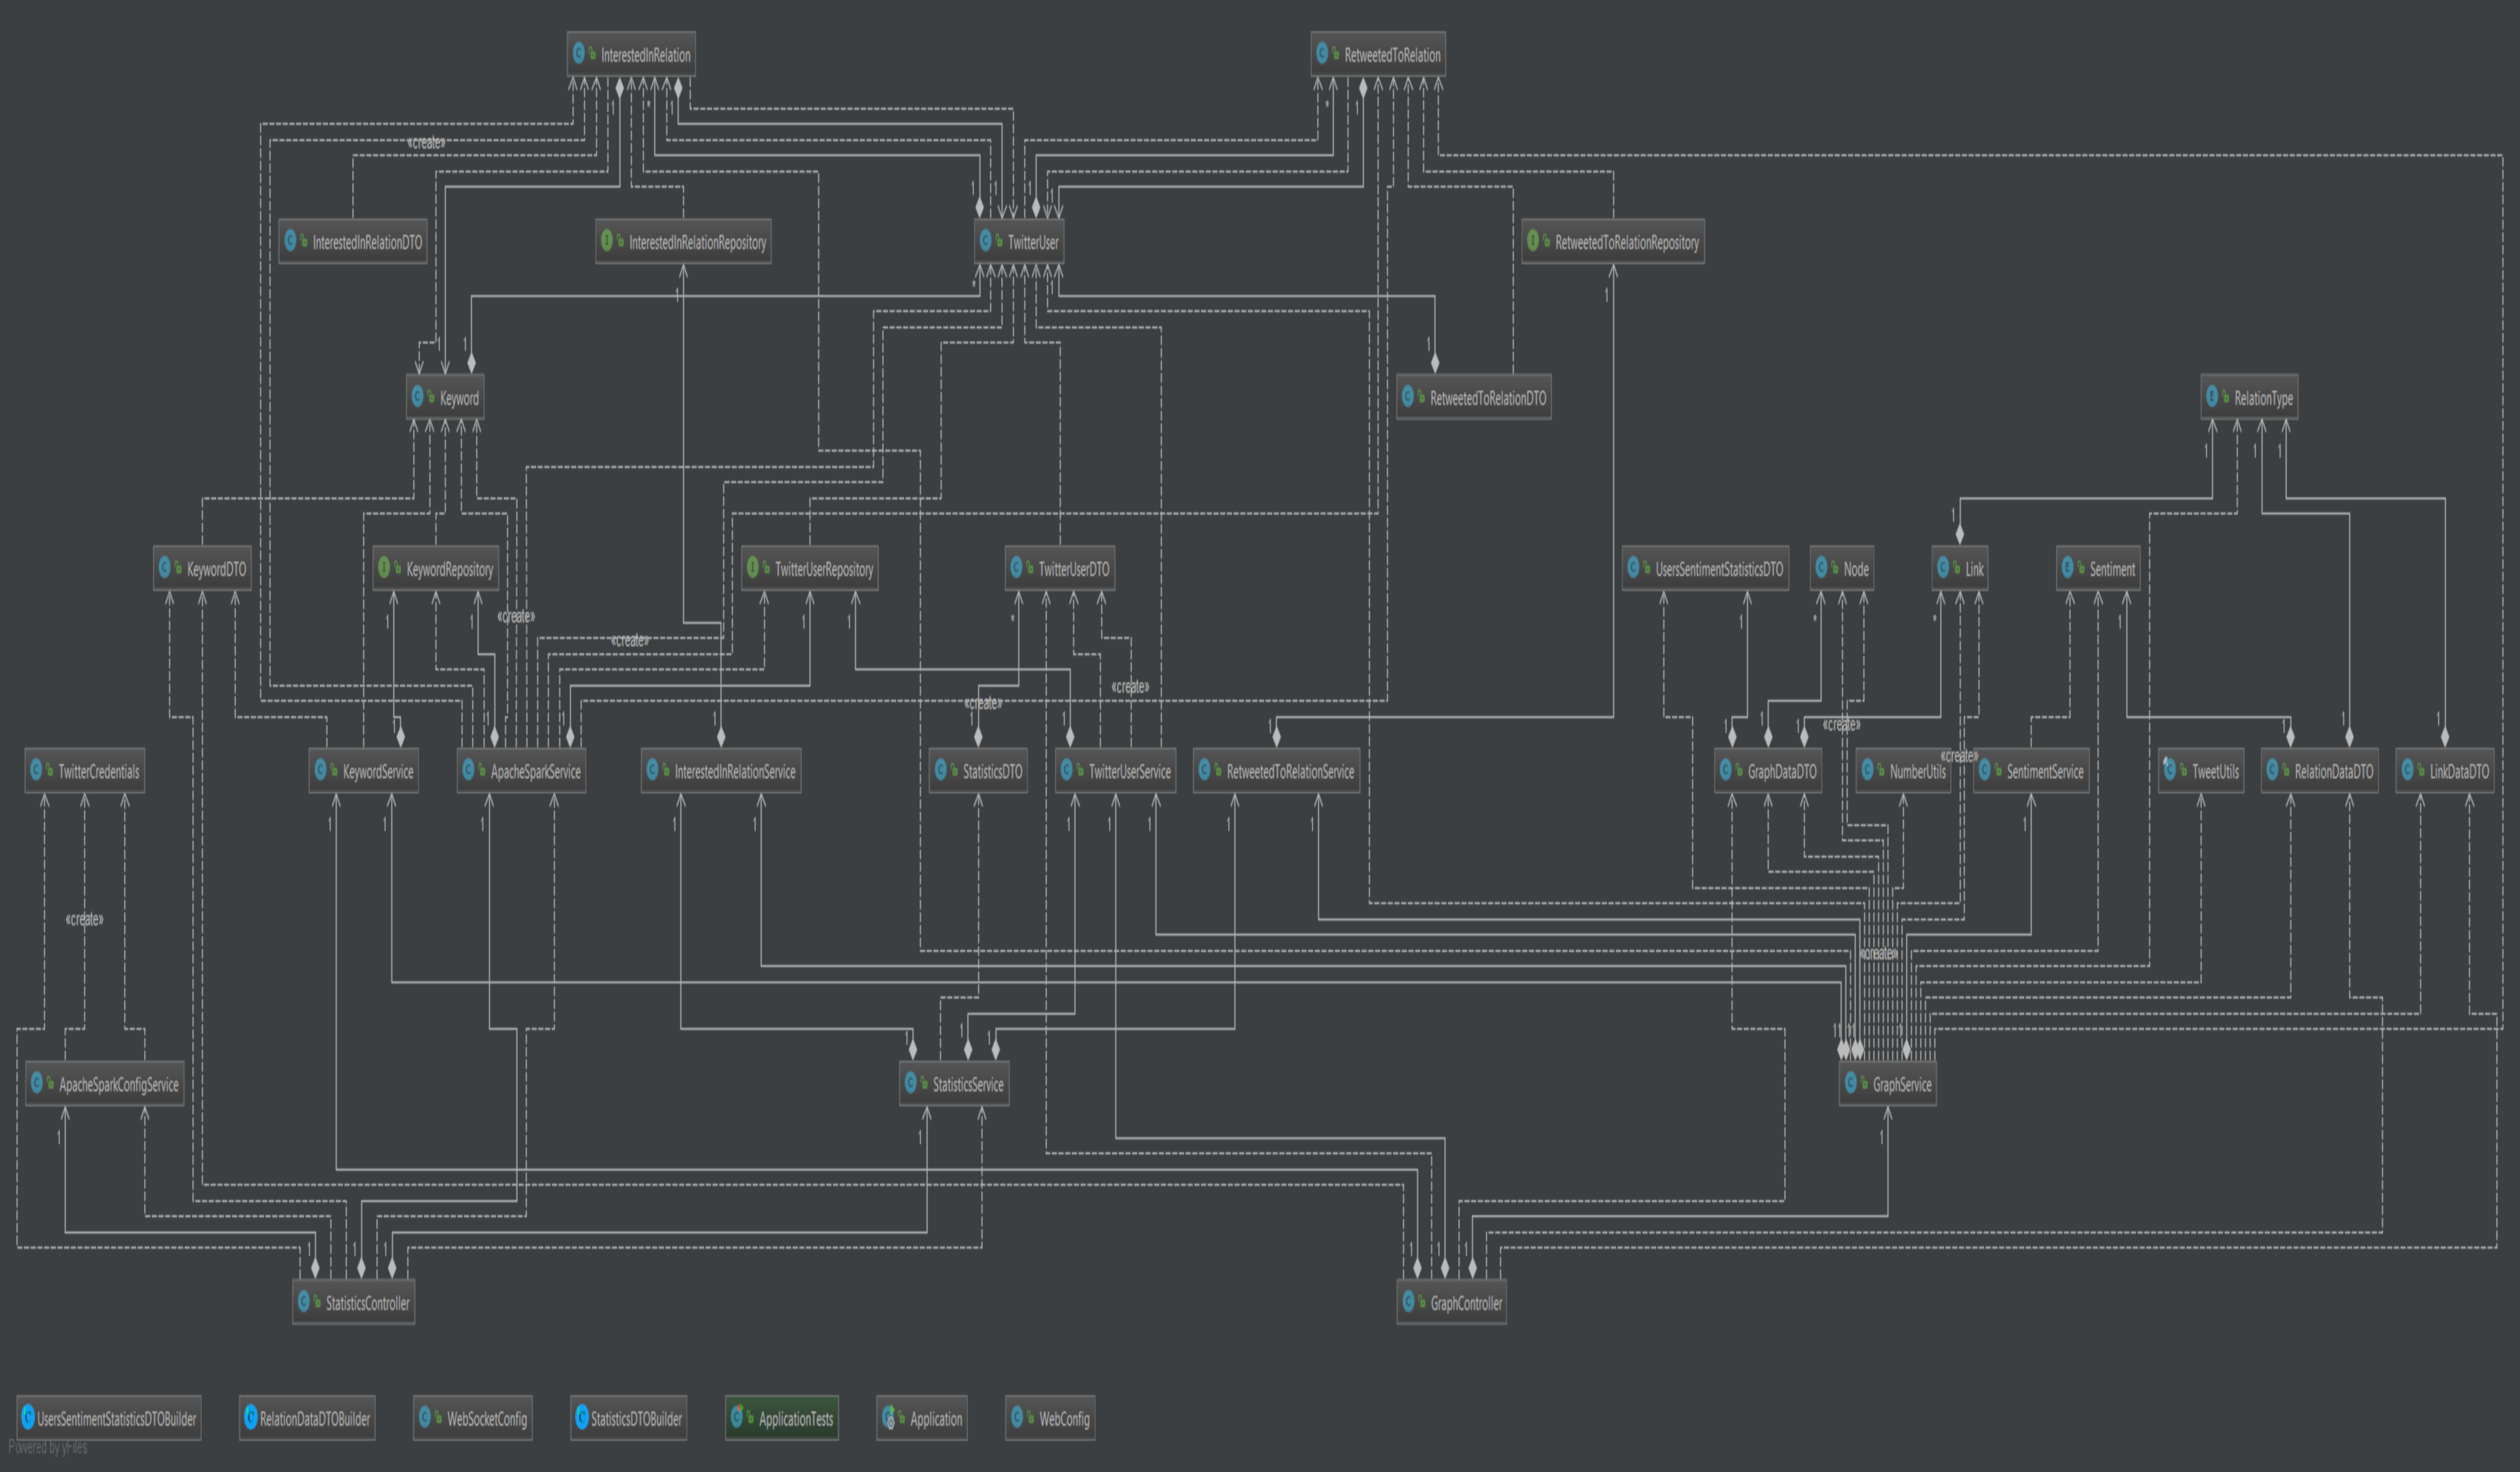
\includegraphics[width=1.5\linewidth, angle=90]{img/twitter_analyser_class_diagram}
	\caption{Przykład zastosowania operacji na strumieniach oraz wyrażenia lambda w kodzie napisanym w języku Java w wersji 8.}
\end{figure}


